\begin{frame}{3D Parametric Curve}
\begin{center}
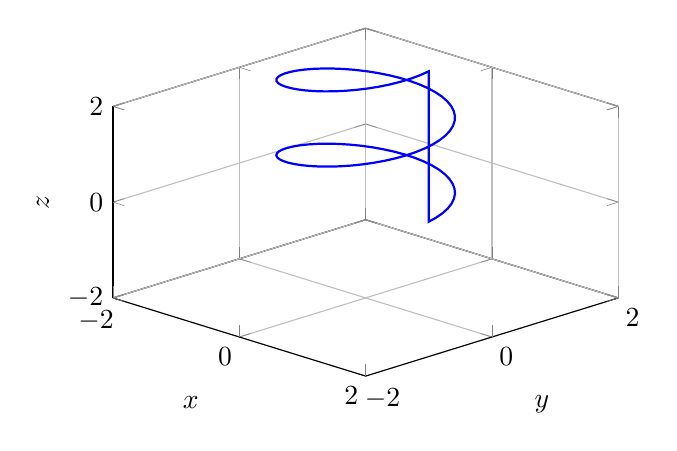
\begin{tikzpicture}
\begin{axis}[
    xlabel={$x$},
    ylabel={$y$},
    zlabel={$z$},
    grid=both,
    xmin=-2, xmax=2,
    ymin=-2, ymax=2,
    zmin=-2, zmax=2,
    width=8cm,
    height=6cm,
    view={45}{30}
]
\addplot3[thick, blue, domain=0:4*pi, samples=100] ({cos(deg(x))}, {sin(deg(x))}, {x/4});
\end{axis}
\end{tikzpicture}
\end{center}

\footnotesize
\texttt{\textbackslash addplot3[thick, blue] (\{cos(deg(x))\}, \{sin(deg(x))\}, \{x/4\})}
\end{frame}